\documentclass[a4paper]{article}
\usepackage{geometry}
\usepackage{multicol}
\usepackage{setspace}
\usepackage{listings}
\usepackage{graphicx}
\usepackage{algorithm}
\usepackage{algpseudocode}
\usepackage{amsmath}
\usepackage{amssymb}
\usepackage{multicol}
\usepackage{float}
\DeclareGraphicsExtensions{.eps,.ps,.jpg,.bmp}
\usepackage{xcolor}
%\setlength{\parskip}{0.5\baselineskip}
\geometry{left=2.5cm,right=2.5cm,top=1.5cm,bottom=2.0cm} 
\title{\textbf{Algorithmn HW11}}
\author{5140379032 JIN YI FAN}
\date{}
\begin{document}
\maketitle
\begin{spacing}{1.3}
%\begin{multicols}{2}
\section*{Problem 16.4}
\begin{multicols}{2}
Disaprove, right is the counter example, in which $s\rightarrow a\rightarrow b\rightarrow t$ and $s\rightarrow a\rightarrow c\rightarrow t$ are both maximum flows.
\begin{figure}[H]
    \centering
    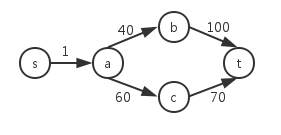
\includegraphics[width=4.5cm]{11-1.png}
\end{figure}
\end{multicols}

\section*{Problem 16.10}
Apply to $G(V,R)$ DFS to get topological sort sequence;
\\Modify Dijkstra Algorithm, Search for most-weighted edge, add to visited edge set until $s$ and $t$ appear on one path, take this path.

\section*{Problem 16.15}
\begin{multicols}{2}
\begin{figure}[H]
    \centering
    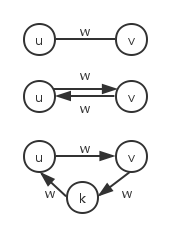
\includegraphics[width=3cm]{11-3.png}
\end{figure}
Transfer single-connected undirected graph to double-connected directed graph with parallel reverse edges.
\\Then add an extra vertex to one of the parallel edges to eliminate parallel edges.
\\Then the minimum weight cut can be transfered to maximum flow, and can be solved by $Ford-Fulkerson$ algorithm and its improved algorithm.
\end{multicols}

\section*{Maxflow with vertex capacities}
\begin{multicols}{2}
\begin{figure}[H]
    \centering
    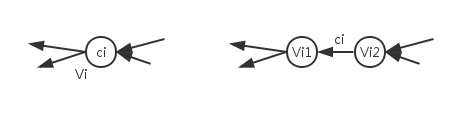
\includegraphics[width=8cm]{11-2.png}
\end{figure}
Break each vertex $V_i$ into two, $V_{i1}$ and $V_{i2}$,  and add one edge between with capacity equals to the origin vertex capacity ($c_i$).
\\The new graph will have $2v$ vertices and $e+v$ edges.
\end{multicols}

\section*{Maximum flow in $\left|E\right|$ steps of augmenting}
We can apply $MPLA$ algorithm described in section 16.5 in the text boos.
\\The $Lemma\ 16.5$ shows it can be limited in $\left|E\right|$ times of augmenting.
%\end{multicols}
\end{spacing}
\end{document}

